\section{Quantitative Violation Semantics}

\paragraph{Motivation for Quantitative Semantics.}
The fundamental limitation of the forward-looking tight satisfaction semantics lies in its binary and prefix-closed nature.
Specifically, the monitoring process halts definitively at the first tight violation, effectively freezing the verdict even if subsequent events in a long-running trace would constitute further breaches.
While computationally efficient for runtime enforcement, this ``first-fail'' approach masks the full history of non-compliance.
It fails to capture cumulative violations or independent failures by multiple agents over time, which is a critical requirement for comprehensive legal or normative accountability.
To address this limitation, one must move beyond simple boolean or blame-set verdicts to a quantitative semantics.
Such an approach measures the ``degree'' or ``count'' of violations over the entire duration of the contract.
Potential methods include cumulative violation counting, weighted penalties, or violation density metrics, all of which provide a more nuanced and legally robust assessment of contract performance.

\paragraph{Determining the Scope of Quantification.}
To count violations cumulatively rather than stopping at the first breach, we must determine which part of the contract is currently ``in force'' at any given step.
A key challenge is defining the temporal window over which violations are aggregated. We identify two primary strategies:
\begin{enumerate}
   \item \textbf{Pre-computing Contract Length ($T$):} One approach is to try to calculate the precise ``duration'' or ``length'' of the contract execution beforehand. If we knew a contract $C$ lasts exactly $T$ steps, we could simply sum the violations over the window $[0, T]$. However, this turns out to be complicated because contracts involving regular expressions (like guards or triggers) or unbounded repetitions ($\repit{C}$) have variable lengths that depend entirely on the runtime input of the agents. The ``length'' is not static; it is dynamic and trace-dependent.
   \item \textbf{On-the-Fly End Detection:} A more flexible alternative is to compute the end of the contract dynamically. At each step, the monitor checks if the current prefix constitutes a ``complete execution'' or ``end'' of the contract before deciding to move to the continuation. This is essentially a greedy or localized version of a ``Best-Split'' logic: as soon as the contract can be considered finished (even with violations), we switch context to the next phase.
\end{enumerate}
In this work, we opt for \textbf{On-the-Fly End Detection} as it allows for a more responsive and adaptable monitoring strategy suitable for runtime verification of dynamic behaviors.

First, we formalize the \textbf{Contract Progress Monitor} (CPM).
This monitor relies on a progression function $\Prog: \Gamma^* \times \cDL \to \cDL$ that, for any finite prefix $\pi$ and a contract $C$, returns the active remaining parts or residual of the contract as  residual contract.
Unlike simple binary monitors, the CPM identifies which specific sub-contract or obligation is currently \emph{in force} given the history of events---distinguishing, for instance, whether a sequential contract $C_1; C_2$ is currently enforcing the initial phase $C_1$ or has progressed to the continuation $C_2$.
Second, we define the \textbf{Quantitative Violation Semantics} to establish how violation scores are calculated based on these residuals.
Finally, we present the \textbf{Quantitative Blame Semantics} and its corresponding automata construction.
By leveraging the structural tracking of the CPM to identify exactly which obligations were active at each step, this framework enables the cumulative counting of violations and the precise attribution of blame to agents over the entire duration of a contract.

\paragraph{Section Plan.}
Similarly to the methodology established in the previous section on forward-looking tight semantics, we structure our investigation of quantitative semantics as follows.
We begin by defining the \textbf{Contract Progress Monitor} function, which serves as the operational foundation for tracking contract evolution.
Next, we formally introduce the \textbf{Quantitative Violation Semantics} to define the counting mechanism for breaches, followed by the construction of the corresponding automata.
Finally, we extend this framework to \textbf{Quantitative Blame Semantics}, detailing how cumulative scores are attributed to specific agents, and conclude with the construction of the quantitative blame monitor.

\subsection{Contract Progress Monitor}
The core of the quantitative framework is the ability to track the state of the contract as it evolves over time. We formalize this using a \emph{progression function} that computes the residual contract after observing a trace prefix.

\begin{definition}[Contract Progression Function]
Let $\Gamma = 2^\Sigma$ be the event alphabet and let $\mathcal{C}$ be the set of all contracts in \cDL extended with a special symbol $\emptc$. The symbol $\emptc$ signals that all parts of the contract have been enforced before (i.e., the contract is effectively empty or fully processed).
The progression function $\Prog: \Gamma^* \times \cDL \to \cDL \cup \{\emptc\}$ reduces the formula on the fly following the timed progress on the trace. It takes a finite trace prefix $\pi$ and a contract $C$ and returns the residual contract.
For the empty trace $\epsilon$, $\Prog(\epsilon, C) := C$.
For a single event step $\trace{A}$ with $A \in \Gamma$, the function is defined recursively on the structure of $C$:

 \paragraph{Literals.}
 For any literal $\ell$:
 \[
 \Prog(\trace{A}, \ell) := \emptc
 \]
Whether the literal is satisfied ($\trace{A} \satt \ell$) or violated ($\trace{A} \violt \ell$), it is consumed by the step $A$. The distinction between satisfaction and violation is handled by the quantitative scoring function, not the structural progression.

 \paragraph{Conjunction.}
 \[
 \Prog(\trace{A}, C_1 \wedge C_2) := \Prog(\trace{A}, C_1) \wedge \Prog(\trace{A}, C_2)
 \]
 With the identity: $\emptc \wedge C' \equiv C'$ and $C' \wedge \emptc \equiv C'$.

 \paragraph{Sequence.}
 For a sequence $C_1 ; C_2$, the progression depends on whether $C_1$ has been fully discharged (reduced to $\emptc$).
 \[
 \Prog(\trace{A}, C_1 ; C_2) := 
 \begin{cases}
   \Prog(\trace{A}, C_1) ; C_2 & \text{if } \Prog(\trace{A}, C_1) \neq \emptc, \\
   \Prog(\trace{A}, C_2) & \text{if } \Prog(\trace{A}, C_1) := \emptc \text{ (immediate hand-over)}.
 \end{cases}
 \]
 Technically, if $C_1$ finishes exactly at step $A$, the residual is $C_2$. If $C_1$ takes multiple steps, we remain in the sequence structure. 

 \paragraph{Reparation.}
 \[
 \Prog(\trace{A}, C_1 \repair C_2) := 
 \begin{cases}
   \Prog(\trace{A}, C_1) \repair C_2 & \text{if } \trace{A} \presat C_1 \text{ (still pending)}, \\
   \Prog(\trace{A}, C_2) & \text{if } \trace{A} \violt C_1 \text{ (failure triggers repair)}, \\
   \emptc & \text{if } \trace{A} \satt C_1 \text{ (success clears all)}.
 \end{cases}
 \]

 \paragraph{Repetition.}
 \[
 \Prog(\trace{A}, C^n) := \Prog(\trace{A}, C) ; C^{n-1}
 \]
 \[
 \Prog(\trace{A}, \repit{C}) := \Prog(\trace{A}, C) ; \repit{C}
 \]

 \paragraph{Guarded Contract ($\guard[re]{C}$).}

 \[
 \Prog(\trace{A}, \guard[re]{C}) :=
 \begin{cases}
   \emptc & \text{if } \trace{A} \satt \guard[re]{C} , \\
   \guard[\Prog_{re}(re')]{\Prog(\trace{A}, C)} & \text{otherwise (guard continues)}.
 \end{cases}
 \]


 \paragraph{Triggered Contract ($\trig[re]{C}$).}
 The trigger activates $C$ once $re$ matches.
 \[
 \Prog(\trace{A}, \trig[re]{C}) :=
 \begin{cases}
   \emptc & \text{if } \trace{A} \violt re \text{ (trigger impossible)}, \\
   C & \text{if } \trace{A} \satt re \text{ (Trigger fires)}, \\
   \trig[\Prog_{re}(\trace{A},re)]{C} & \text{if } \trace{A} \presat re.
 \end{cases}
 \]
 Where the regular progress function $\Prog_{re}: 2^\Gamma \times \cDL_{re} \to \cDL_{re} $ is defined only when $\trace{A} \presat \re$ (where $\trace{A}$ is the trace consisting of the single event $A$).
 We do not need to use $\epsilon_{re}$ as we did for the contract as $\epsilon$ is already defined in the syntax of regular expression, with $\Prog_{re}(\trace{A},\epsilon):= \epsilon$ 
 \paragraph{Atomic regular expressions}
 For a set of actions $A \in \Gamma$ we have:
$Prog_{re}(\trace{A}, A') := \epsilon.$ 
  
 \paragraph{Concatenation}
For $\re \cdot \re'$, the progression is defined as:
\[
\Prog_{re}(\trace{A}, \re \cdot \re') := 
    \Prog_{re}(\trace{A}, re) \cdot re'.
\]

\paragraph{Union}
For $re \mid re'$, the progression is defined by distinguishing cases based on violation:
\[
\Prog_{re}(\trace{A}, re \mid re') := \begin{cases} 
\Prog_{re}(\trace{A}, re') & \text{if } \trace{A} \violt re ,\\
\Prog_{re}(\trace{A}, re) & \text{if } \trace{A} \violt re' ,\\
\Prog_{re}(\trace{A}, re) \mid \Prog_{re}(A, re') & \text{otherwise}.
\end{cases}
\]

\paragraph{n-repition}
For $\re^n$, with $n \in \mathbb{N}^*$ the progression is defined as:
\[
\Prog_{re}(\trace{A}, re^n) := \Prog_{re}(\trace{A},re)\cdot re^{n-1}.
\]


\paragraph{Operator $+$}
For $\re^+$, the progression is defined as:
\[
\Prog_{re}(\trace{A}, re^+) := \Prog_{re}(\trace{A}, re) \mid \Prog_{re}(\trace{A},re)\cdot re^+.
\]

Moving up for the special case of single event traces, for $\pi = \trace{A} \circ \pi'$ with
$A \in \Gamma$ the first event and $\pi' \in \Gamma^*$ the remaining suffix. Then:
\[
  \Prog(\trace{A} \circ \pi', C) :=
  \begin{cases}
    \emptc & \text{if } \Prog(\trace{A}, C) = \emptc, \\[4pt]
    \Prog\bigl(\pi',\,\Prog(\trace{A}, C)\bigr) & \text{otherwise}.
  \end{cases}
\]
\end{definition}



\begin{lemma}[Termination of Progression Function]
  \label{lem:prog-termination}
  For every finite trace prefix $\pi \in \Gamma^*$ and every contract $C$ in \cDL, the progression call $\Prog(\pi, C)$ terminates.  
  Moreover, it performs at most $\lvert \pi \rvert$ recursive steps on the trace.
  \end{lemma}
  
  \begin{proof}[Proof sketch]
  For a prefix $\pi = \trace{A} \circ \pi'$, the definition first computes the one-step residual $\Prog(\trace{A}, C)$.  
  This computation always terminates since it proceeds by structural recursion on strict subparts of~$C$, or yields $\emptc$ directly in the literal case.
  
  If $\Prog(\trace{A}, C) = \emptc$, the entire evaluation stops immediately because the residual contract is empty and no further events in $\pi'$ need to be processed.
  
  If $\Prog(\trace{A}, C) \neq \emptc$, the progression continues with the suffix $\pi'$.  
  Since $\pi'$ is strictly shorter than $\trace{A} \circ \pi$, each recursive descent reduces the length of the remaining prefix by exactly one.  
  
  Because $\pi$ is finite, at most $\lvert \pi \rvert$ such descents are possible.  
  The process therefore always terminates, either earlier when the residual becomes $\emptc$, or after consuming the entire prefix.  
  No infinite recursion can occur.
  \end{proof}

  \begin{example}[Progression for $C=\repit(\obl{\PAY})$]
    \label{ex:prog-repit}
    
    Consider the contract
    \[
      C_3 := \obl[1]{\PAY}\ \repair\ \obl[1]{\PAYF}.
      \]
  
  We study the progress of the function on the first trace, where the first event satisfy the contract:
  $\pi= \trace{A_1, A_2}$, where:
  $A_1=\{\PAY^1, \PAY^2\}$, and $A_2=\{\OCC^1\}$. The result is summarized in Fig.\ref{example:prog-repitc}
    \boxalignfigure{\resizebox{0.7\textwidth}{!}{%
    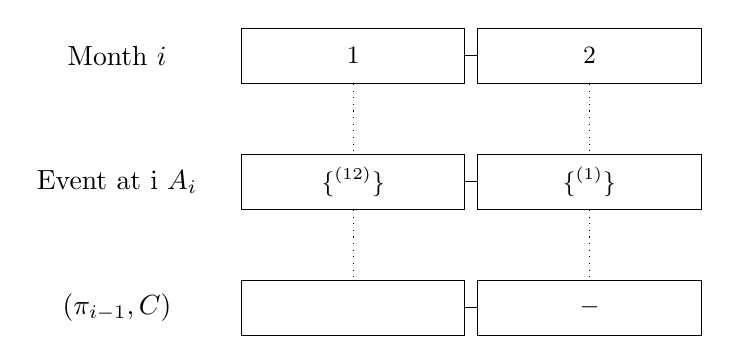
\begin{tikzpicture}[y=1.6cm,x=3.0cm]
    
      \tikzset{
        cell/.style={
          draw, rectangle, text width=26mm,
          minimum height=7mm, align=center, font=\small
        }
      }
    
      % Labels
      \node at (0,0)   {Month $i$};
      \node at (0,-1)  {Event at i $A_i$};
      \node at (0,-2)  {$\Prog(\pi_{i-1},C)$};
    
      % Row 1: time
      \node[cell] at (1,0) (t1) {$1$};
      \node[cell] at (2,0) (t2) {$2$};
    
      % Row 2: events
      \node[cell] at (1,-1) (e1) {$\{\PAY^{(12)}\}$};
      \node[cell] at (2,-1) (e2) {$\{\OCC^{(1)}\}$};
    
      % Row 3: residuals
      \node[cell] at (1,-2) (r1) {\emptc};
      \node[cell] at (2,-2) (r2) {$-$};
    
      % Arrows
      \draw (t1)--(t2);
      \draw (e1)--(e2);
      \draw (r1)--(r2);
    
      % Vertical alignment
      \draw[dotted](t1.south)--(e1.north);
      \draw[dotted](e1.south)--(r1.north);
    
      \draw[dotted](t2.south)--(e2.north);
      \draw[dotted](e2.south)--(r2.north);
    
    \end{tikzpicture}
    }}
    {Progression on $ \obl[1]{\PAY}\ \repair\ \obl[1]{\PAYF}$ with a trace for which a no reparation is not required}
    {example:prog-repitc}
    {\vspace{8pt}}{\vspace{-12pt}}


    We study the progress of the function on a second trace $\pi'$, where the first event of this trace does not satisfy the contract:
    

    \end{example}
    \todo{regexp norm, repeat}
